%!TEX root = ../thesis.tex
%*******************************************************************************
%****************************** Second Chapter *********************************
%*******************************************************************************

\chapter{General physical properties 2D materials \label{chap:3}}

\ifpdf
    \graphicspath{{Chapter3/Figs/Raster/}{Chapter3/Figs/PDF/}{Chapter3/Figs/}{Chapter3/Figs/Vector/}}
\else
    \graphicspath{{Chapter3/Figs/Vector/}{Chapter3/Figs/}}
\fi

In this thesis, the properties of materials are divided into a preliminary and an advanced category, where the latter will be presented in the next chapter as the main results of this thesis. In this chapter, I will focus on the preliminary properties of 2D materials, namely structural, electronic, vibrational and mechanical properties. These properties are considered as test calculations and knowledge which the advanced properties are closely relied on. They are composed both of my original calculations and results from literatures. An emphasis will be made on the characteristic properties of 2D materials that are different for 3D cases.

\section{Structural properties}
\subsection{Layer structure}

As discussed in the \fullref{chap:1}, layered bulk materials have a close relationship with 2D materials. The strong anisotropic structure in the former results in the layer concept in the latter, and a single layer of a layered bulk material is a 2D material. This anisotropic nature is attributed to the weak interlayer bonds and the strong intralayer bonds. Van der Waals (vdWs) interactions \cite{vdws} are the main types of these weak interlayer bonds. vdWs interactions are the attraction and the repulsion between atoms or molecules entities caused by dipole-dipole, dipole-induced dipole and instantaneous induced dipole-induced dipole forces. The definition is sometimes extended to include all dispersion forces between molecules.  For 2D materials, vdWs interactions become important as the number of layers is larger than one; that is few-layer materials with typical less than ten layers. They also belong to the family of 2D materials since the thickness of the materials still small for quantum confinements to dominant their roles. As in its layered bulk counterpart, a few-layer system is a stacks of monolayers that hold together through vdWs forces. When no other bonding types present, interlayer vdWs interactions determine all the change brought by going above single layer, and its impact on the electronic structure can be significant. For example, from monolayer to bilayer, the linear dispersion relation of energy $E$ and momentum $k$ around the $K$ k point evolves into parabolic-like spectrum\cite{Partoens2006,Mak2010}. 

\begin{figure}[htbp!] 
\centering  
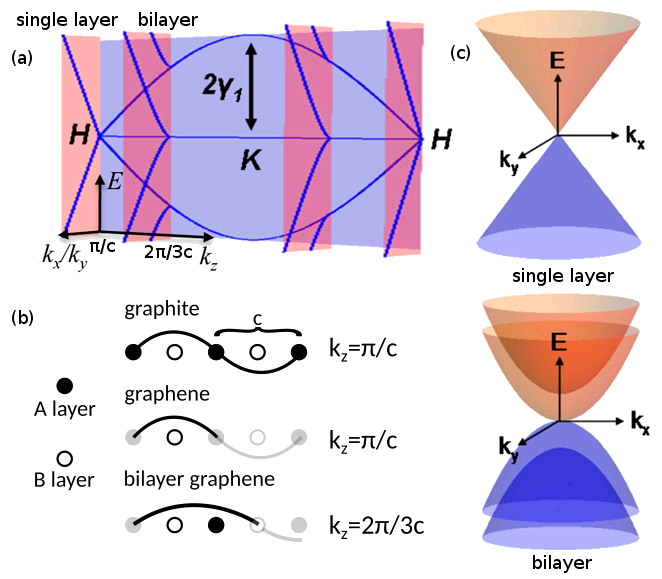
\includegraphics[width=0.9\textwidth]{gra_band.png}
\caption{(a) Energy-momentum dispersion relations of single layer and bilayer graphene as approximated by plane intersections of 3D graphite dispersion relation and (b) their 3D dispersion relations around the $K$ k point. (c) Wavelength matching of graphite to single layer and bilayer graphene. Image adapted from: \cite{Mak2010}. }  
\label{fig:gra_bands}
\end{figure} 

In \autoref{fig:gra_bands} (a), the dispersion relation of graphite along the z direction, that is the HKH line in the Brillouin zone, is shown on the blue plane. This direction is perpendicular to the graphite layers. Because of the interlayer interaction and the quantum confinements, in few-layer system, the finite thickness limits the number of wave vectors that standing waves can take.  Therefore, if only the intralayer and interlayer interactions between the nearest neighbour atoms were considered, the dispersion relations in few-layer systems can be approximated as those on the cross-section of red planes with the 3D graphite dispersion relation, see \autoref{fig:gra_bands} (a).  These planes are perpendicular to the z direction and intersect with the HKH line at limited points. This is called the zone-folding of dispersion relations\cite{saito1998physical}. These points are illustrated in \autoref{fig:gra_bands} (c). Under the condition that quantum confinements at few-layer system require the wave functions vanish at the imaginary layer right outside the surface of the system, the systems will have well-defined wave vectors. Then, the dispersion relations of graphene and bilayer graphene will be on the red planes intersect the HKH line at $k_z=\pi/c$ and at $kz=2(\pi/3c)$, respectively.  Having the knowledge of 3D band structure of graphite, we can approximate the dispersion relation of few-layer systems in this way. As a result, as shown in red plane in \autoref{fig:gra_bands} (a) and their 3D version in \autoref{fig:gra_bands} (b), graphene has linear dispersion relations and bilayer graphene has parabolic-like two bands that come from each layer. Moreover, the bilayer structure will never pass through the H point where graphene has passed to have linear dispersion relations. This is because of the standing waves in bilayer will have a wave vector $k=2(n \pi/3c)$, where $n$ is a positive integer: 1, 2, ... , n. This will never equal to $\pi/c$ for any integer number of $n$. More generally, systems with an even number of layers will not have the linear dispersion relation, and vice versa for system have an odd number of layers. Further, if other interactions were considered, an overlap of bands those touch each other in (c) would happened\cite{Partoens2006}. This overlap increases with the number of layers. Eventually in graphite, maximum overlap is reached.


\begin{figure}[htbp!] 
\centering  
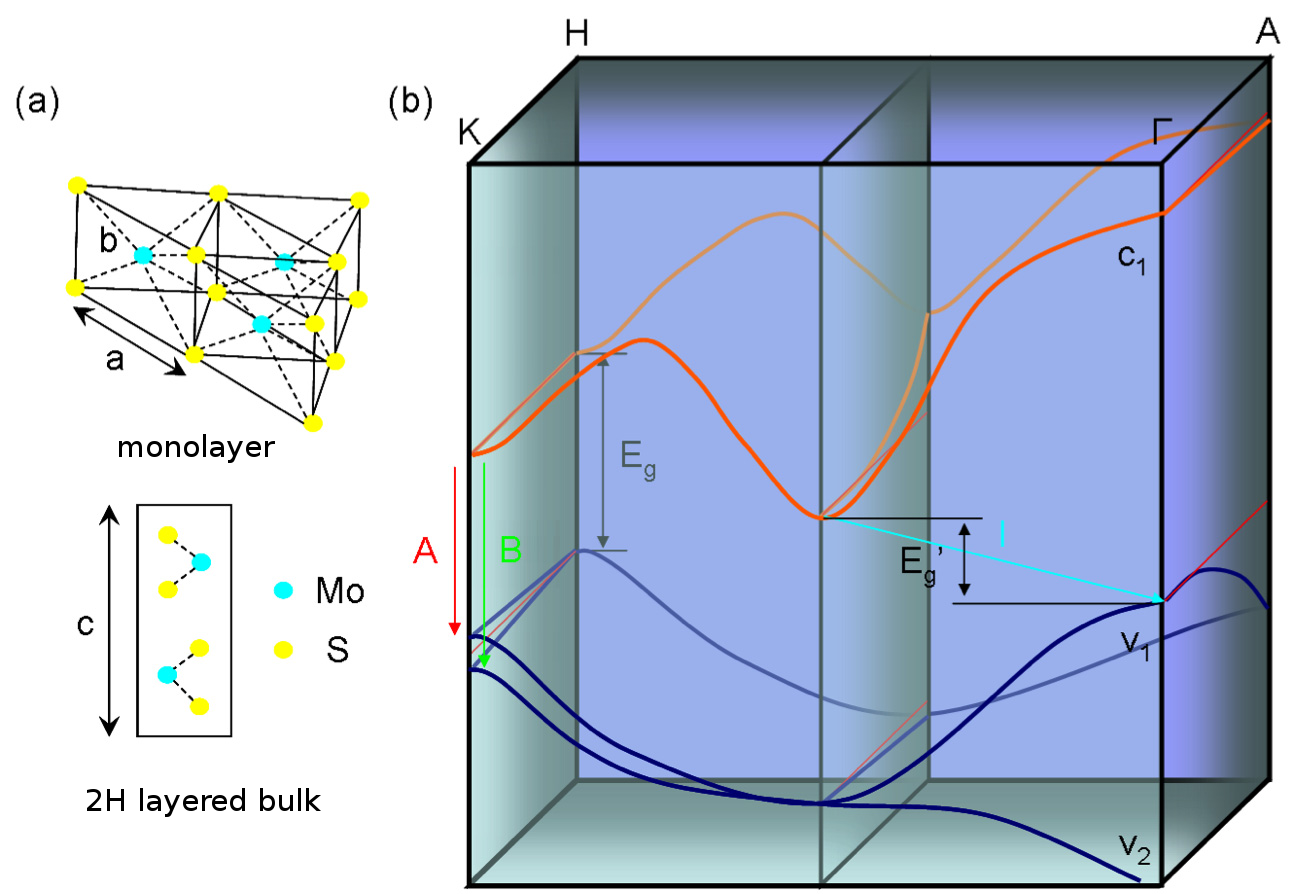
\includegraphics[width=0.8\textwidth]{mos2_band.png}
\caption{Energy-momentum dispersion relations of MoS$_2$ as plane intersections of 3D dispersion relations. Image adapted from: \cite{Mak2010b}. }  
\label{fig:mos2_band}
\end{figure} 

Another example of the importance of interlayer interactions in few-layer 2D materials is for MoS$_2$. As mentioned in the \fullref{chap:1}, as going from layered bulk to monolayer, MoS$_2$ transforms from an indirect band gap to a direct one. Here again, we can make use of zone-folding scheme to approximate the band structure of the monolayer from that of the layered bulk. The monolayer and the layered bulk structure of 2H phase are shown in \autoref{fig:mos2_band} (a). In figure (b), let us focus on the planes parallel to the page that passing through the K$\Gamma$ line and the HA line (simply call them K$\Gamma$ plane and HA plane below). Same as the previous discussed graphite, 2H layered bulk MoS$_2$ has two layers per unit cell. Therefore, according to the standing wave arguments that we have used for the graphene case above, HA plane represents the monolayer. $E_g$ and $E\prime_g$ are the band gaps of the monolayer and the layered bulk structures. Here, not only the magnitude of the band gap is increased as going from layered bulk to monolayer, the character of the band gap has changed as well. It is clearly shown that this is due to the band edges shifting. VBM at $\Gamma$ and CBM at the middle of $\Gamma$K line are brought more closer as going from monolayer to layered bulk. This corresponds to the widening of band width and it is coming from the splitting of the VB and CB when more and more layers interact with each other through the interlayer interactions. Therefore, band gap in the layered bulk are defined by these two band edges, which in the monolayer was defined by band edges at $K$. In contrast to this, the band edges at the $K$ are not effected too much by the interlayer interaction to make a difference. So why the band edges react differently to the interlayer interactions? If we look into the orbital composition of the band edges, we will find the ones have widened the most, i.e. VBM at $\Gamma$, have the largest contribution from S $p_z$ and Mo $d_{z^2}$ orbitals. These out-of-plane orbitals vertically orientate to the plane thus have maximum overlap with the others from an adjacent layer. Therefore, band splitting is more profound for these band edges to widen the band width. Whereas both of the CBM and VBM at $K$ are largely composed of S $p_x$ and $p_y$ orbitals and Mo $d_{xy}$ and $d_{x^2-y^2}$ orbitals. All of them are in-plane orientated orbitals thus have limited effect from interlayer interactions\cite{Padilha2014}.

\subsection{sp hybridization}

After discussed about the layered structure and the importance of interlayer interaction, let us look into some details of the in-plane structures and how sp hybridization gives rise to various structures for 2D materials. When atoms come together form bonds, the orientations of bonding orbitals are decisive for the final structure. The sp hybridization is a good example of this.  It mainly exists in three different variants: sp, sp$^2$ and sp$^3$, see \autoref{fig:sp_hybrid}. The hybridization index $n$ in sp$^n$ stands for the relative amount of p character in the resulting hybridized orbital. For example, sp$^2$ has 1/3 s character and 2/3 p character. Hybridized orbitals tend to maximized their distance to reduce the energy raised by the repulsion of electrons. As shown in \autoref{fig:sp_hybrid}, this results in tetrahedral structure of sp$^3$ orbitals as in diamond, trigonal planar structure of sp$^2$ orbitals as in graphene or graphite and linear structure of sp orbitals as in ethyne molecules.  This is, for example, useful to explain the buckled structure of graphane and fluorographene. Because of sp$^3$ character developed as a results of the fourth electrons are bonded with H or F atoms, buckling appears in these systems. 

\begin{figure}[htbp!] 
\centering  
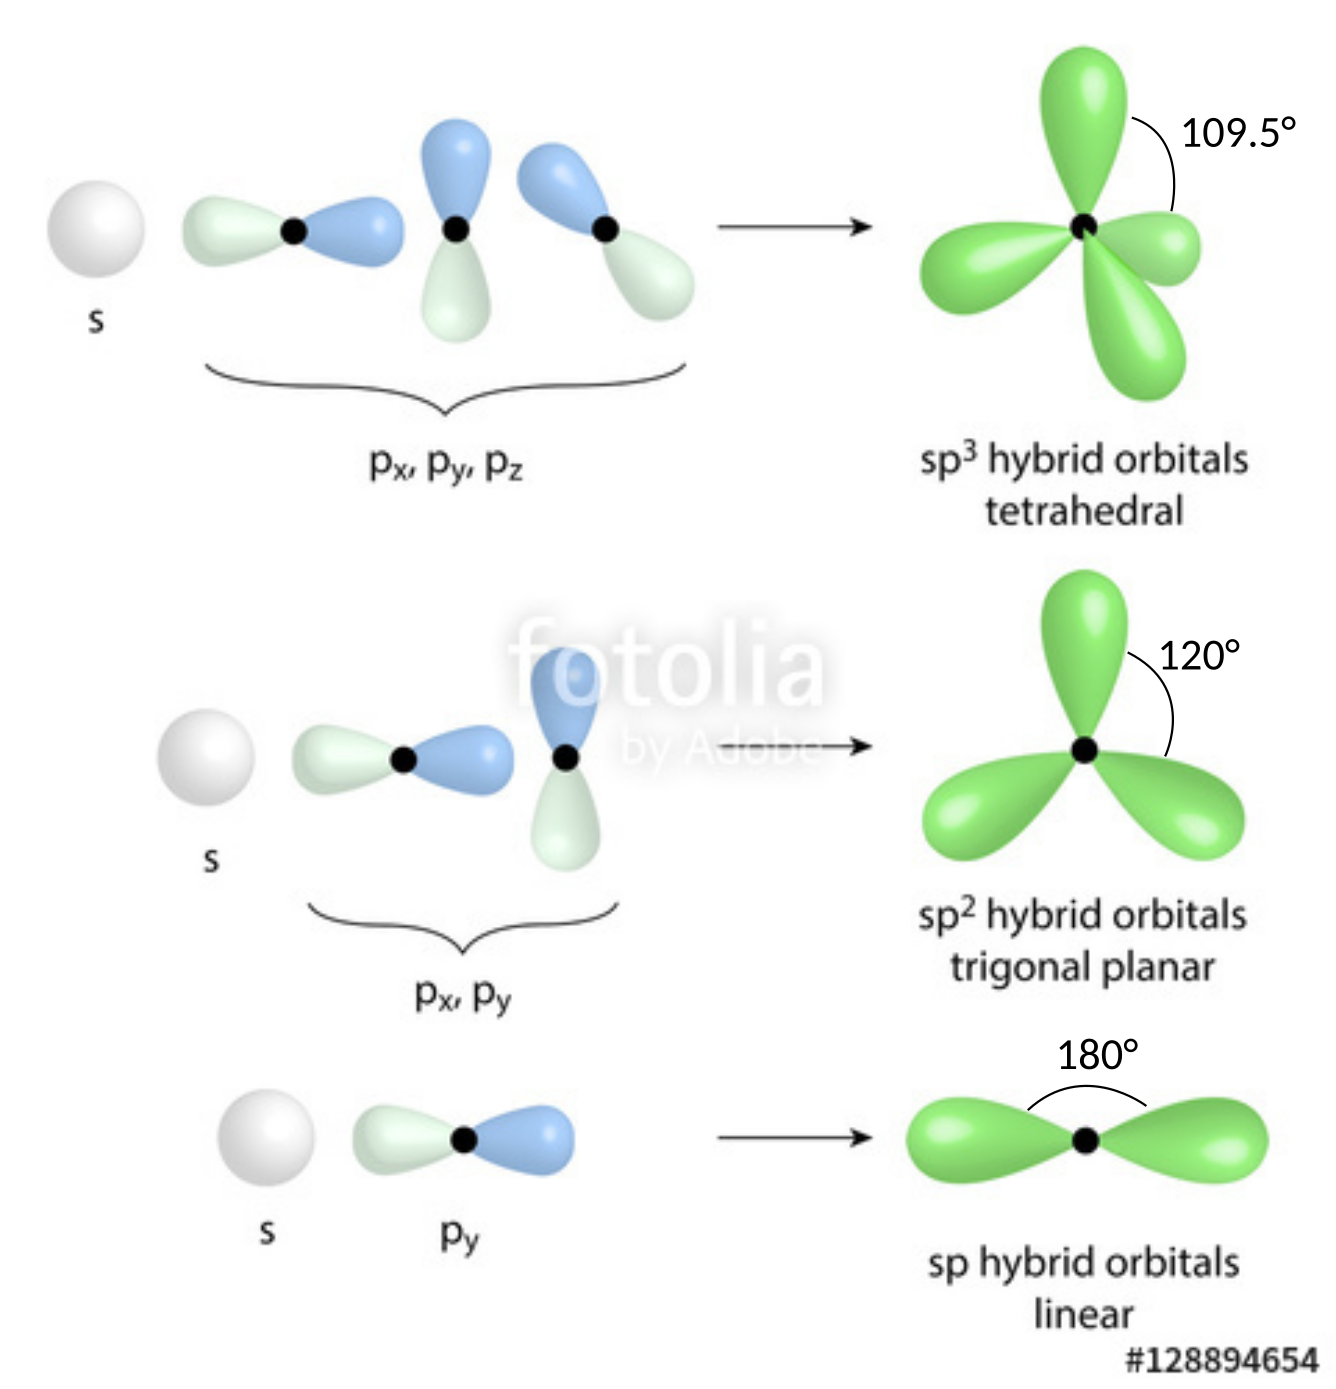
\includegraphics[width=0.8\textwidth]{sp_hybrid.png}
\caption{Three types of sp hybridized orbitals. Image adapted from: \cite{sp_hybrid}. }  
\label{fig:sp_hybrid}
\end{figure} 

{\huge \textcolor{red}{check the english below}}

\citet{coulson1949} generalized the relation of bond angle with $n$ as follows:

\begin{equation}\label{coulson}
1=-\sqrt{n_1n_2}~cos\theta_{12}, 
\end{equation}

where $\theta_{12}$ is the bond angle between orbital 1 and 2. The bond angle can be measured in structure after relaxation simulations, yet we still need one more constrain to solve \autoref{coulson} for hybridization index $n$ if orbital 1 and 2 have different $n$. This constrain is that, in the case of carbon atom, the total portions of all s orbitals should equal 1, while it should be 3 for the p orbitals. With these knowledge, \autoref{coulson} can be solved, and each bond from one atom can be assigned with a unique $n$. This formula is useful to determine the s and p fractions of the bonds. For example, $\theta_{12}=90^o$ gives $n\rightarrow\infty$, which means it is a pure p orbital; $\theta_{12}=120^o$ gives $n=2$, that is a sp$^2$ hybridized bond. Generally, wider bond angle corresponds to large s contribution: bond angles are ordered as sp > sp$^2$ > sp$^3$. Of course, \autoref{coulson} is more useful when the bond angle takes the values other than those three types of hybridized bonds mentioned, then it can be used to explain the resulting geometry.


\section{Electronic properties}

Electronic properties is one of the first feature we usually would like to know about the new materials. Not only it is because semiconductor and metal have different roles in the applications, but also because the details of the electronic structure set the direction towards which further exploration should be carried out. One example for this from my experience is that from monitoring the electronic structure variations under a strain we had predicted how the mobility of the carrier can be tuned. This will be discussed in the later chapter. Therefore, it is important to understand this property of a new material to fully reveal its potentials. Electronic properties usually characterized by band structure (BS) and density of states (DOS). These calculations are standard calculations in common first-principles codes where all consequent calculations start. After solving the Kohn-Sham equation with properly defined cut-off energy, k points etc., we will have the eigenenergy of each state that indexed with k point in the Brillouin zone and band.  DOS is a count of such states at specific energy. BS is the plot of eigenenergy verse the line in Brillouin zone that connects high symmetry k points.  2D material has vast variation of electronic properties. From semimetallic graphene to semiconducting MoS$_2$ and to insulating BN. We have already seen these in the \fullref{chap:1}. The purpose of this section is to point out some of the interesting electronic properties of some of the 2D materials. We will start with a brief introduction to the electronic properties of graphene.

\subsection{Graphene}

As mentioned before, orbitals in graphene are sp$^2$ hybridized. Each one of these sp$^2$ orbitals, coloured in green in \autoref{fig:gra_bond}, is composed from s, p$_x$ and p$_y$ orbitals. The p$_z$ orbital, coloured in yellow in the figure, is left unchanged. One $sp2$ hybridized orbital with another one from adjacent atom form strong $\sigma$ bond, while $p_z$ orbitals form $\pi$ bonds. It may look like an alternative single and double bonds between atoms, actually according to the Clar's theory, the bond order, i.e. the number of chemical bonds between a pair of atoms, in graphene is 4/3 and it is uniform\cite{Wassmann2010}.

\begin{figure}[htbp!] 
\centering  
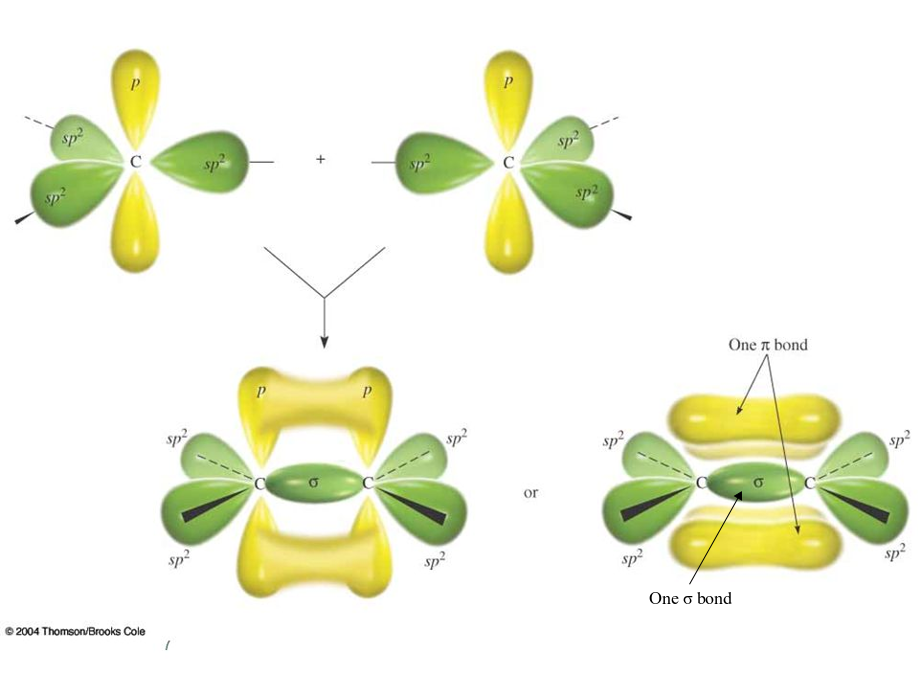
\includegraphics[width=0.7\textwidth]{double_bond}
\caption{The formation of $sp^2$ $\sigma$ and $p_z$ $\pi$ double bond. Image source: \cite{gra_bond}. }  
\label{fig:gra_bond}
\end{figure} 

Every atom has same local environment, however, adjacent atoms are not equivalent. They belong to different hexagonal sublattices $A$ and $B$ as indicated with blue and yellow colors in \autoref{fig:gra_lat}. $a_1$ and $a_2$ are the basis vectors in real space connecting equivalent lattice sites. $b_1$ and $b_2$ are the basis vectors in reciprocal space connecting equivalent k points. The hexagon in the reciprocal space is the first Brillouin zone where all inequivalent k points are contained. These k points associate with different parallel lines of atoms and thus their directions in the reciprocal space are associate with different directions in the real space. The k wave vectors near the $\Gamma$ point have longer wave length, while those at the boundary of the first Brillouin zone have a wave length that is two times the unitcell dimension on that direction. For example, the most interesting k point for graphene is the $K$ and $K'$ points. These directions correspond to the $a_1$ and $a_2$ directions in real space. It is only at these k points in the Brioulloin zone, the antibinding and bonding $\pi$ band touch each other. Addition to this, as we have discussed in the introduction the Dirac cones will form around theses k points. 

\begin{figure}[htbp!] 
\centering  
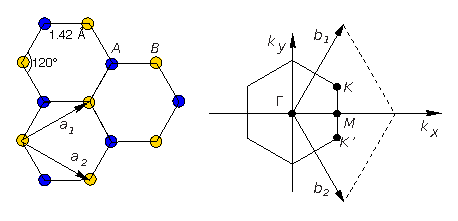
\includegraphics[width=0.8\textwidth]{gra_lat.eps}
\caption{Graphene lattice and its Brillion zone. Image source: \cite{CastroNeto2009}. }  
\label{fig:gra_lat}
\end{figure} 

As compared to $\pi$ bond, $\sigma$ bond originate from strong overlap of $sp^2$ orbitals. The interaction is so strong that the splitting of bonding and antibonding orbitals are large. Which makes the $\sigma$ bonds orbitals deep in energy, or in other word, makes it strong and difficult to break. This feature contributes the most to the mechanical strength of graphene. On the other hand, $p_z$ orbitals are less overlapped. This makes the $\pi$ bond energy close to Fermi level, i.e. the highest occupied state. Therefore, they contribute the most to the electronic properties of graphene.  


\subsection{Dirac cone and symmetry}

We have seen that graphene, silicene and germanene have an interesting electronic structure: Dirac cone. We also have listed the consequences of having such feature: high mobility, massless carrier etc.. In this section, we will discuss the symmetry condition for the existence of Dirac cones. This knowledge is useful to discover more materials with Dirac cone. 
\begin{figure}[htbp!] 
\centering  
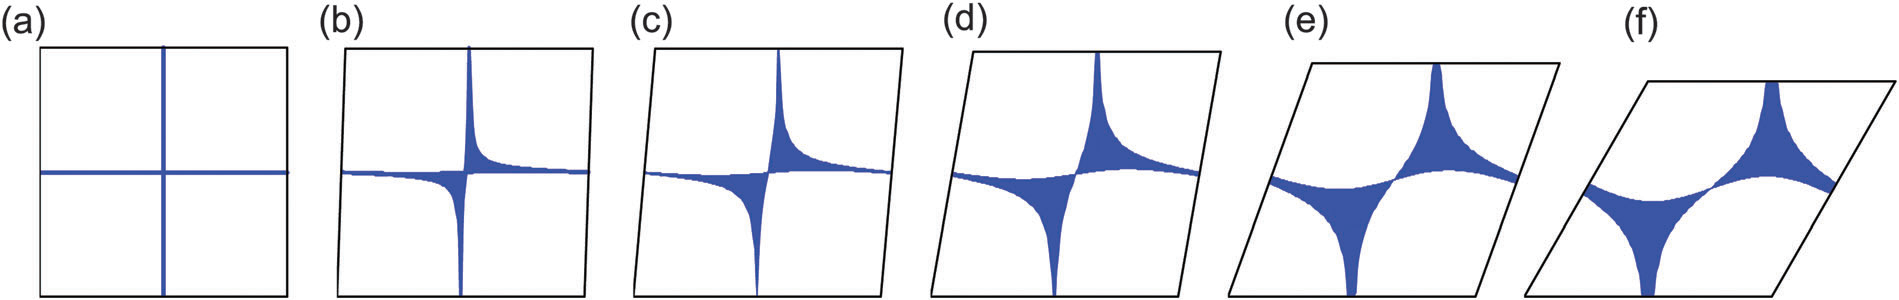
\includegraphics[width=0.95\textwidth]{dirac_hs.png}
\caption{Possible positions of second atom (blue area) to guarantee the existence of Dirac cones as going from (a) square lattice to (f) hexagonal lattice. The first atom is located at the corners of the unit cell. Image source: \cite{Liu2013}. }  
\label{fig:dirac_hs}
\end{figure} 
According to von Neumann-Wigner theorem, the space-time inversion symmetry is crucial for the existence and protection of Dirac cones\cite{Wang2015b}. It is a combination of space inversion and time reversal symmetries. These two are equally important and has to act simultaneously for the possible formation of Dirac cones. More restrict condition that guarantee the existence of Dirac cones has to deal with relations of hopping integrals\cite{Hasegawa2006,Liu2013}. It is from the \citet{Liu2013}'s study that it revealed the hexagonal lattice has the most favourable structure to form Dirac cones. The probability decreases as one goes from a hexagonal lattice to a square lattice, as shown in \autoref{fig:dirac_hs}.

\subsection{Examples: 2D h-BN, 2D MoS$_2$ and graphene}
\begin{figure}[htbp!] 
\centering  
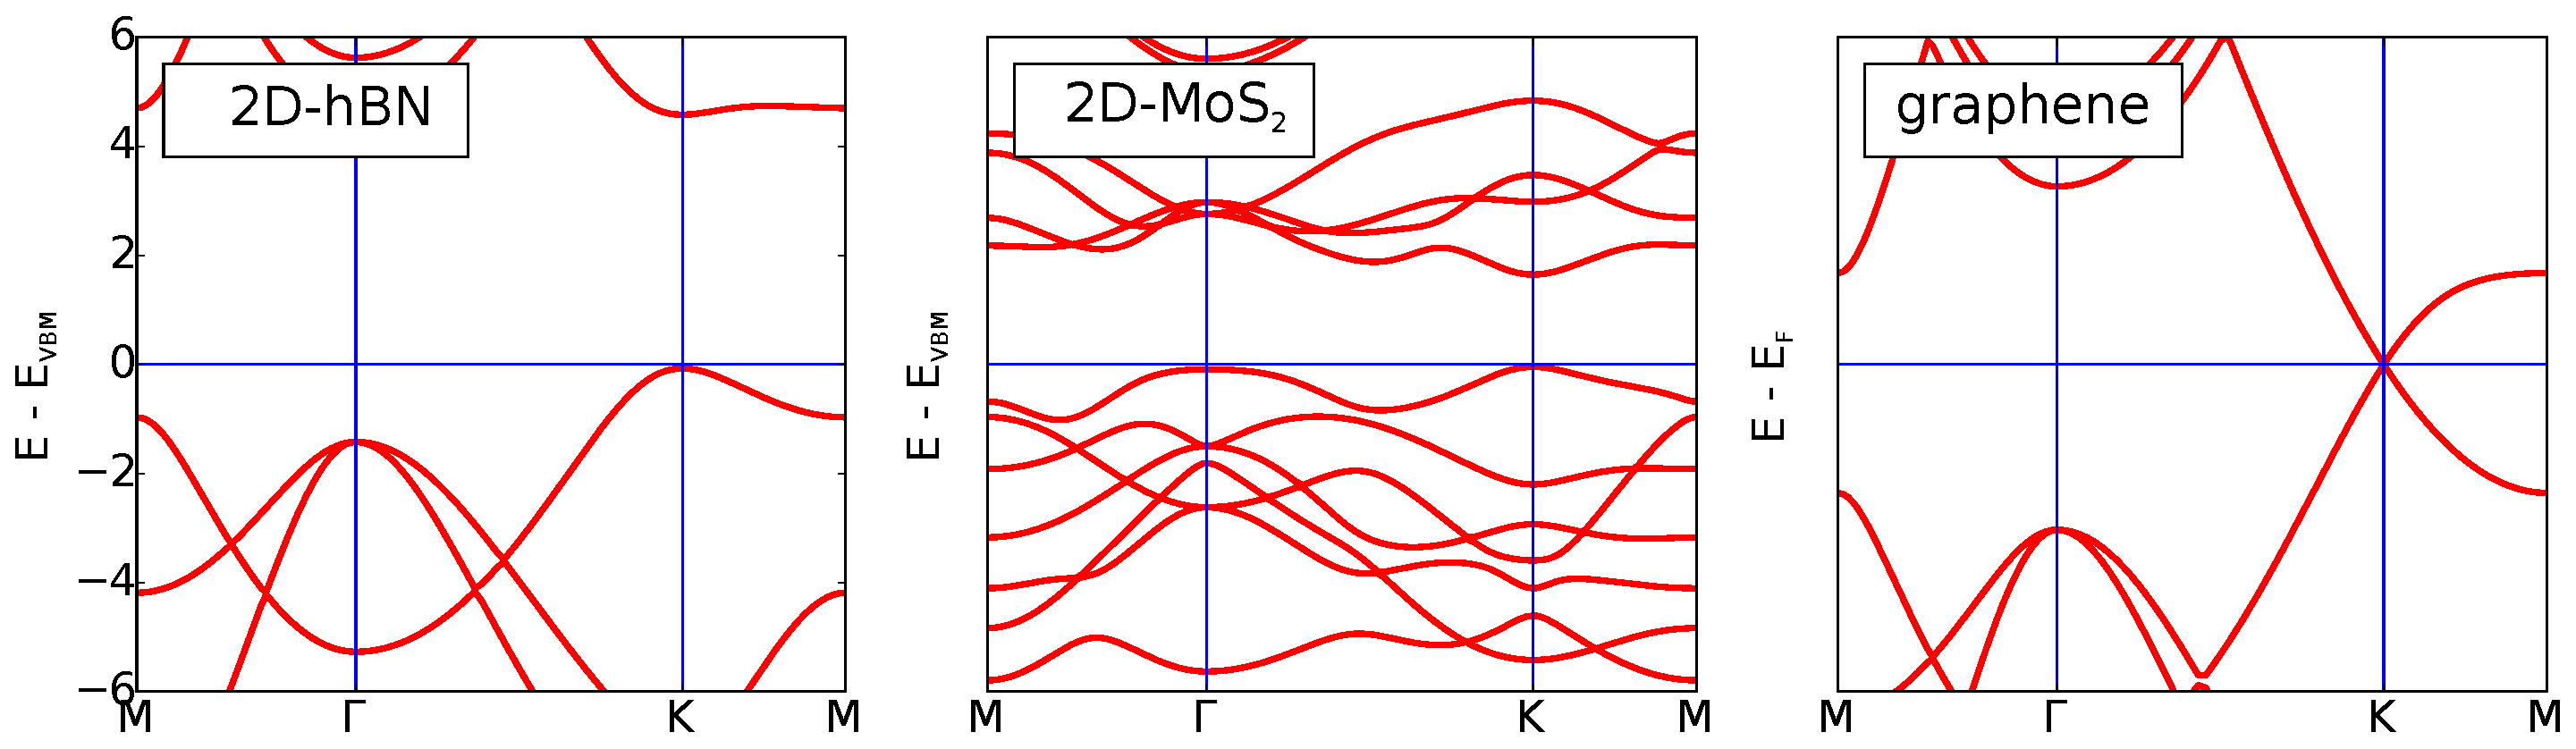
\includegraphics[width=\textwidth]{bss.eps}
\caption{Electronic band structures of 2D-hBN, 2D-MoS$_2$ and graphene. }  
\label{fig:bss}
\end{figure} 
Three typical examples of the band structures of 2D materials are shown in \autoref{fig:bss}. The 2D h-BN is an insulator due to a large band gap in the ultraviolet range, therefore it is suitable to serve as dielectric layer in an electronic device. The 2D TMDs have a band gap ranging from 1.0-2.5 eV which is in the visible and the near infrared range of light, therefore, it is suitable for optoelectronic devices applications. Furthermore, we can see as we compare the dispersion curves along the M$\Gamma$ and K$\Gamma$, the electronic structures are generally the same on these paths which correspond to different crystallographic directions. This means that the materials in the figure are highly isotropic, thus we would expect the same for the physical properties. In the results chapters of this thesis, we will see some new 2D materials that are highly anisotropic. Their discoveries enrich the features of the physical properties of 2D materials.

\section{Vibrational properties}

The force on an atom can be calculated from the wave functions evaluated from DFT thanks to the Hellmann-Feynman theorem. When searching for the equilibrium geometry of the materials, one basically is trying different positions of atoms to find a geometry that minimized all the forces. This usually is the first thing to do for a new materials, since different codes, implementations and, more importantly, different functionals will give different results. Despite the fact that the difference is usually small, unrelaxed geometry will have residual forces on atoms. This is particularly important when vibrational properties are concerned. Vibrational properties are characterized through the energy (usually expressed in terms of frequency) verse vibrational wave vector dispersion relations.  In crystal,  all atoms have their equilibrium positions that consist with the lattice points. Atoms vibrate around these equilibrium positions. The vibrational modes are quantized into phonons. Each phonon represent a periodic, collective vibration with well-defined vibrational mode and wave vector. The forces ($F$) resort the atoms when they deviate from their equilibrium positions can be calculate from DFT either by introducing small displacement or from perturbation theory. Then, force constants, $\Phi$, can be constructed by monitoring the forces change through the displacements, $u$, of atoms in the following way:

\begin{equation}
\Phi_{i\alpha,j\beta}= \frac{\partial F_{j\beta}}{\partial u_{i\alpha}},
\end{equation} 

where the $i,j$ indices are the labels for atoms, $\alpha,\beta$ are the Cartesian directions: $x$, $y$ and $z$. The Fourier transformation of the force constants at wave vector $\mathbf{q}$ is the dynamical matrix $D(\mathbf{q})$ that related to the frequency of the phonon through eigenvalue problem:

\begin{equation}\label{eqa:w_q}
\omega^2(\mathbf{q},n)\mathbf{e}(\mathbf{q},n)=D(\mathbf{q})\mathbf{e}(\mathbf{q},n),
\end{equation}

where $\omega$ is the frequency of the phonon in mode $n$ having a $\mathbf{q}$ wave vector, and $\mathbf{e}(\mathbf{q},n)$ is the eigenvector\cite{Ackland1997,Parlinski2011}.  These modes of phonons are categorized into two main branches, depending on whether atoms in the unit cell are vibrating in-phase (acoustic mode) or out-of-phase (optical mode). For polar materials, polarized atoms vibrate with respect to each other can interact with light, it is why these types of vibrations are called optical modes. Further, considering the directions of the wave ($\mathbf{e}$) and vibration ($\mathbf{q}$), the modes subcategorized into transverse optical (TO) modes and transvers acoustice (TA) modes: ($\mathbf{q} \perp \mathbf{e}$), longitudinal optical (LO) and longitudinal acoustic (LA) ($\mathbf{q} \parallel \mathbf{e}$). These modes are all in-plane vibrations for 2D materials. For such a case, another direction is also important, namely the $\mathbf{c}$ lattice vector direction perpendicular to the 2D plane. Therefore, special modes exist: out-of-plane transverse optical (ZO) and out-of-plane transverse acoustic (ZA) ($\mathbf{q} \perp \mathbf{e}$ and $\mathbf{q} \parallel c$). The total number of acoustic modes is three, that of optical modes is 3N-3, where N is the total number of atoms in the unit cell. 


\subsection{Example: monolayer MoS$_2$}

Let us now take an example of layered bulk and monolayer MoS$_2$ to highlight some of the important details of phonon dispersion relations. A vibrational modes comparison between layered bulk and monolayer MoS$_2$ is presented in \autoref{fig:mos2_ph} (a). First of all, the number of atoms in the unit cell reduces from 6 to 3 from layered bulk to monolayer. Therefore, the number of the optical modes will be reduced as well from 15 in the layered bulk to 6 in the monolayer. In the \autoref{fig:mos2_ph} (a) we see, as being transformed to the monolayer, how each of some modes merges with another one that only different by whether vibration in each layer is in-phase or out-of-phase. Secondly, the appearance of a characteristic feature of phonon disperions for layered bulk and 2D materials: the quadratic ZA mode (flexural mode). It is usually linear in 3D bulk materials because of strong interlayer interactions. Whereas in layered bulk the interlayer interactions are weak and that is absent in 2D materials, therefore, it will cost less energy for the out-of-plane vibration thus make this mode soft. As shown in \autoref{fig:mos2_ph} (b), phonon with longer wave length, i.e. around $\Gamma$, in ZA mode has smaller frequency or energy. This means this mode is easier get excited at low temperature and forms ripples which can be often observed in 2D materials. The formation of ripples is crucial for 2D materials to be stable at finite temperature. Lastly, in the projected DOS, it is shown the projections of mode eigenvetors to in-plane (XY) and out-of-plane (Z) components. The modes with Z components, i.e. ZO$_1$, ZO$_2$ and ZA, contribute the most to the Z projections, and vice versa for the XY components. 

\begin{figure}[htbp!] 
\centering  
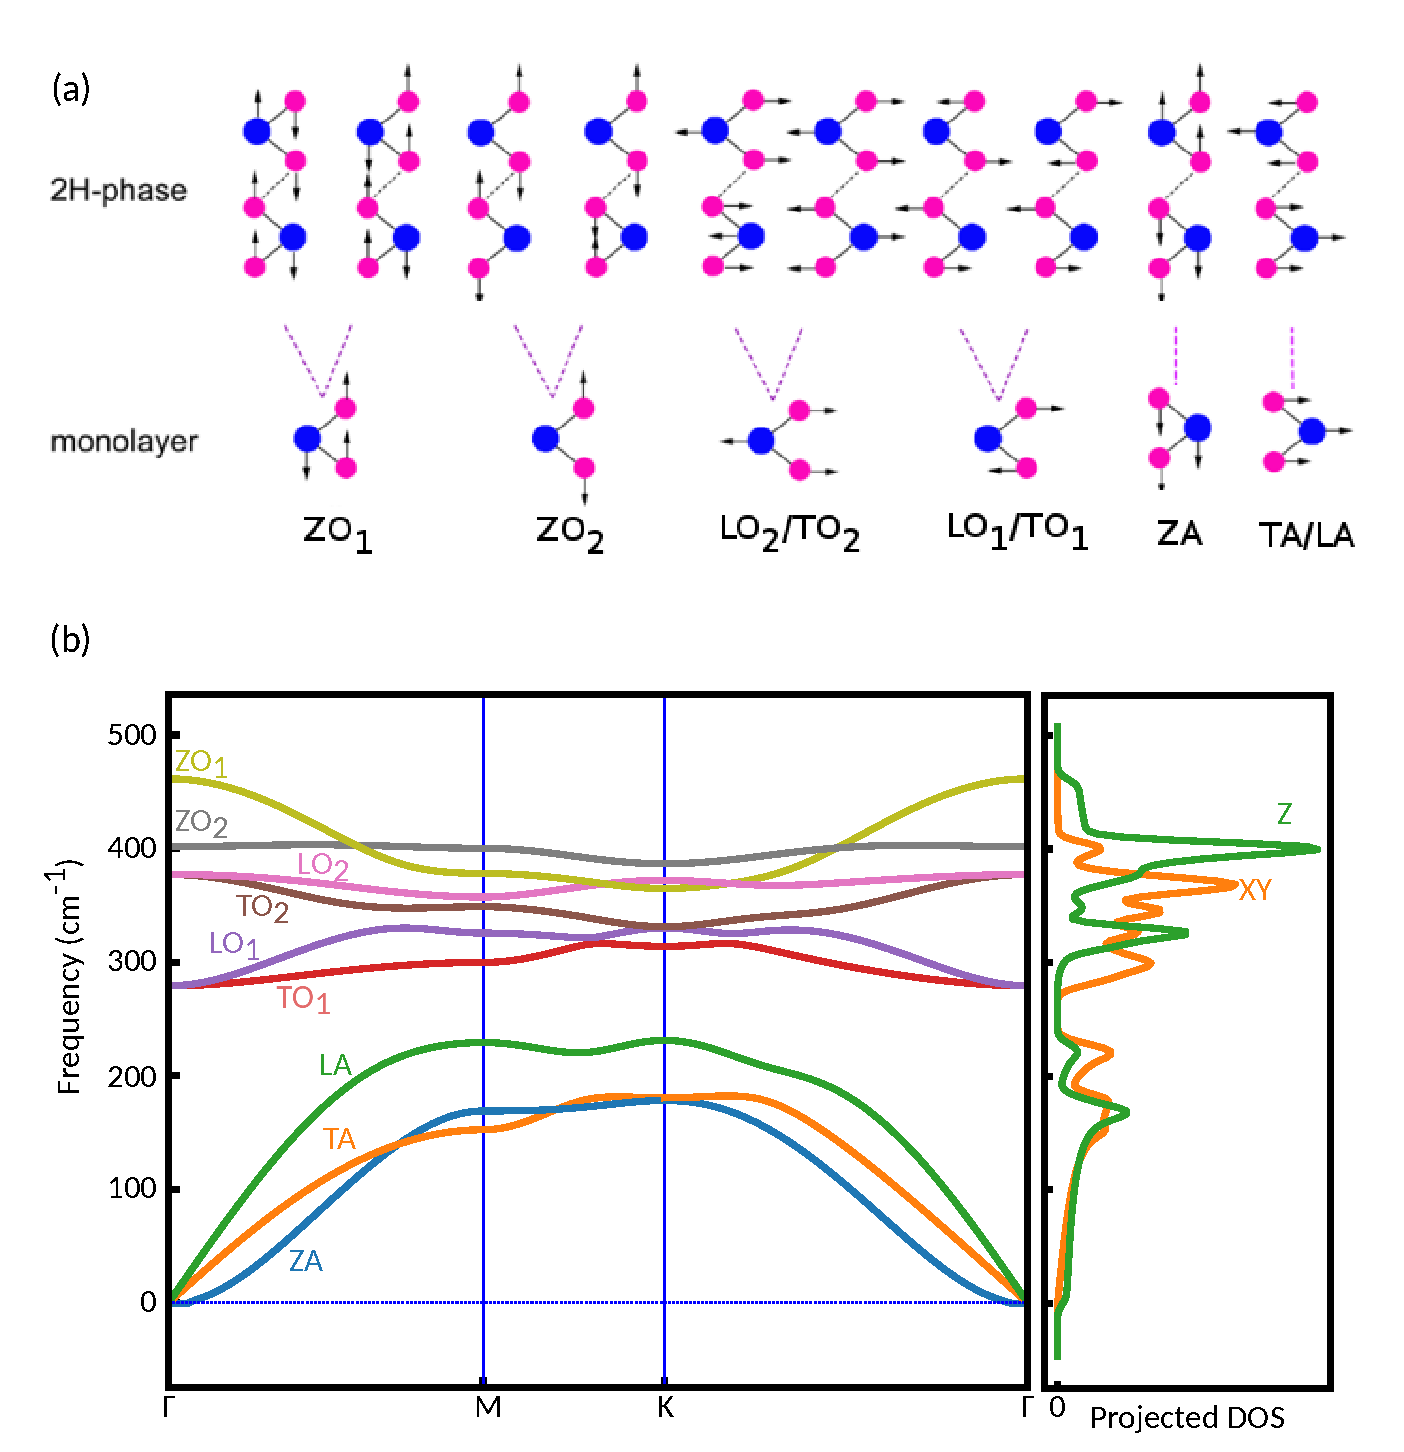
\includegraphics[width=0.8\textwidth]{ph_mos2.eps}
\caption{(a) phonon modes of layered bulk (first row) and monolayer MoS$_2$ at $\Gamma$ q point. (b) phonon dispersion and DOS of monolayer MoS$_2$.}  
\label{fig:mos2_ph}
\end{figure} 


\subsection{Dynamic stability from phonon dispersion}

One of the most important outputs of phonon dispersion is to verify the dynamical stability of the structure. An unstable structure is usually indicated with imaginary frequencies of its phonon dispersion in a portion of its Brillouin zone, see \autoref{fig:img_band} for example. 


\begin{figure}[htbp!] 
\centering  
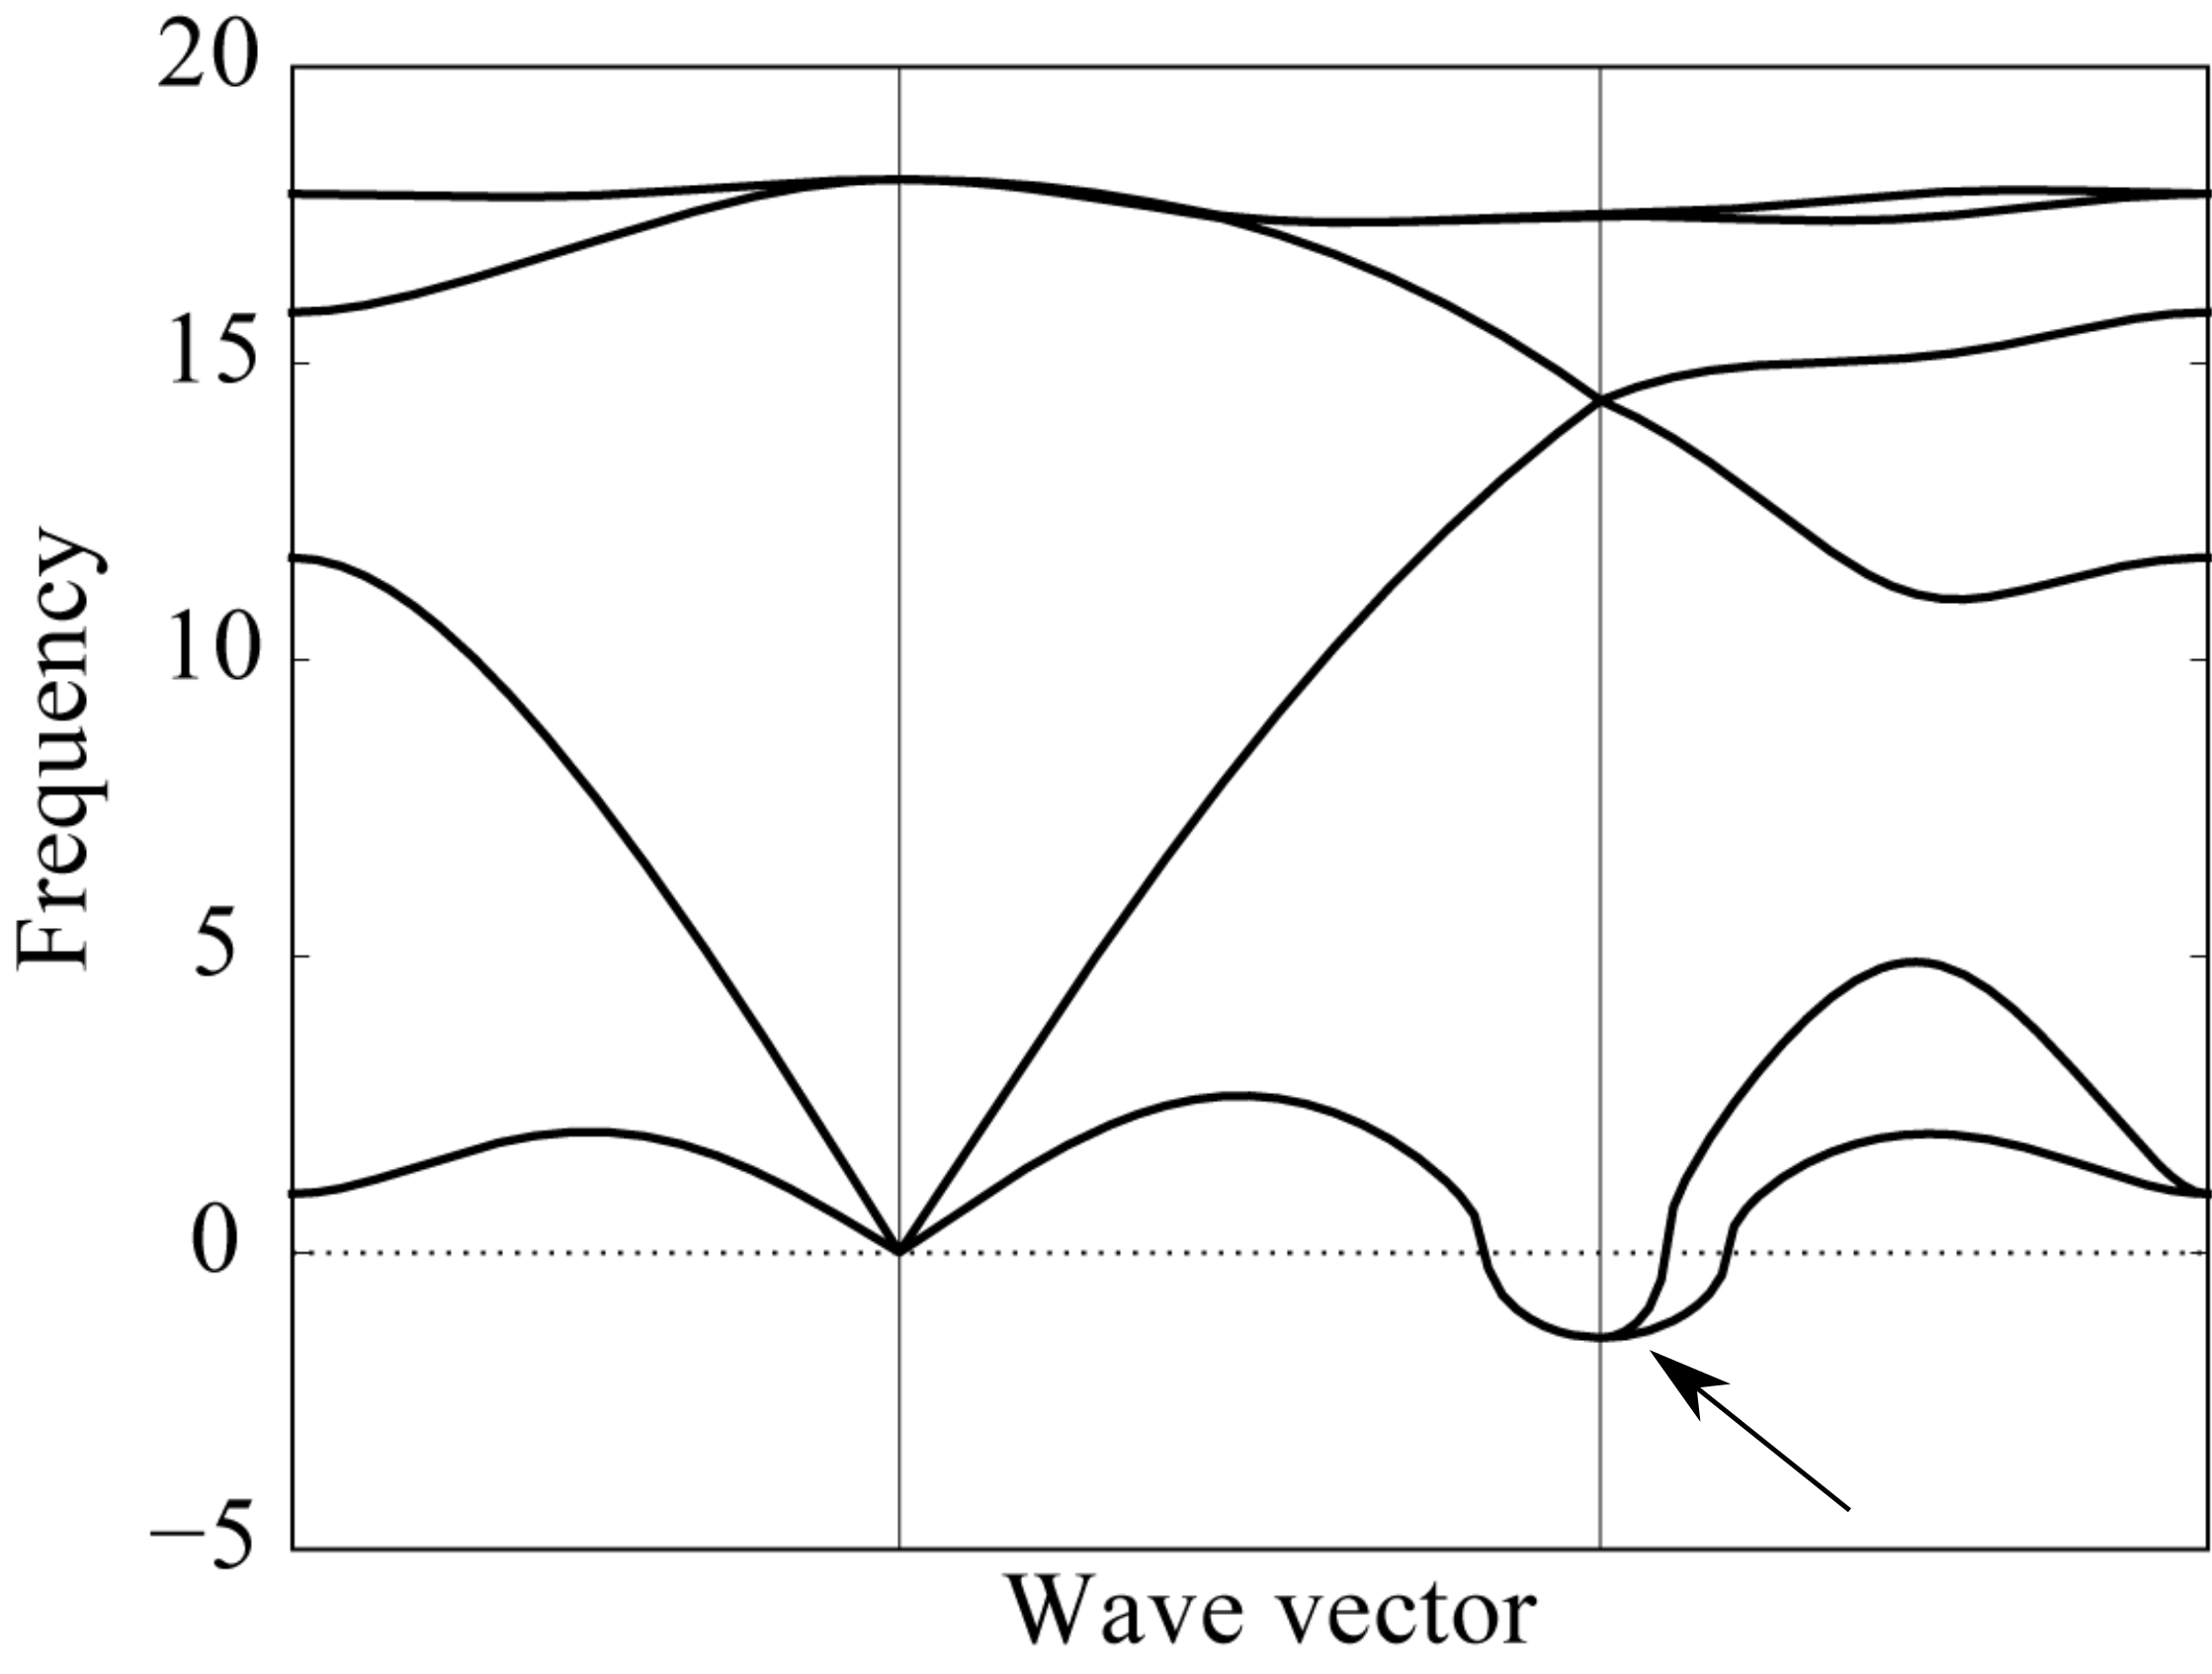
\includegraphics[width=0.5\textwidth]{img_band.png}
\caption{ Imaginary frequencies are shown as negative frequencies in a phonon dispersion plot.}  
\label{fig:img_band}
\end{figure} 

\begin{figure}[htbp!] 
\centering  
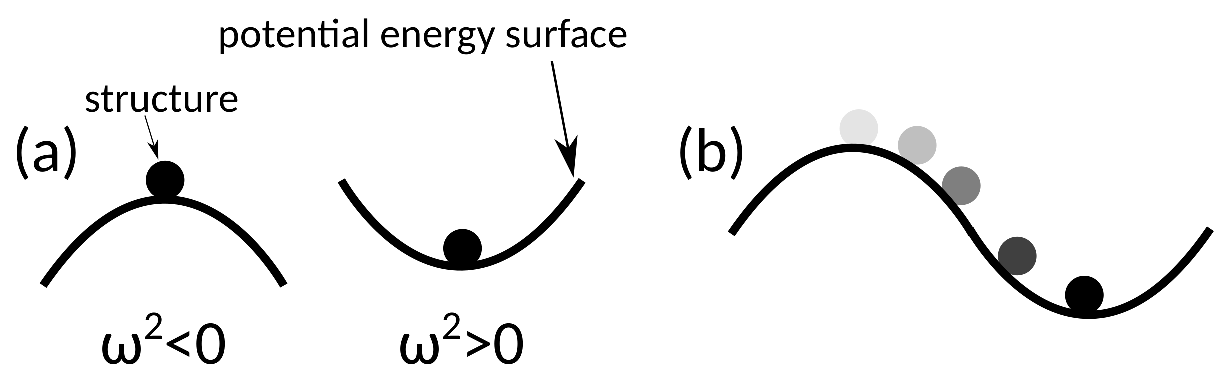
\includegraphics[width=0.7\textwidth]{fre_ima.eps}
\caption{ (a) A structure at the convex (left) and concave (right) of the PES. (b) Searching for stable structure (phase transition).}  
\label{fig:fre_ima}
\end{figure} 

Now let us try to understand it and make use of it to convert the unstable to a stable structure. Consider a relaxed structure in which forces on all atoms are vanished. This could be on a convex or on a concave of the potential energy surface (PES), see \autoref{fig:fre_ima}. Note that, in both situations the forces, the derivative of the PES curves, are zero. Therefore, both situations can occur when the structure is relaxed only following the forces. In the case of PES convex, the dynamical matrix $D(\mathbf{q})$ will have negative components because the direction of the force is same as the displacement. We have seen from \autoref{eqa:w_q}, $D(\mathbf{q})$ is related to the square of frequency $\omega$, hence imaginary frequencies are the only solutions. However, structure with imaginary frequency near $\Gamma$ q point not necessarily means it is not stable. Since a large supercell consist of multiples of unit cell is typically used to do phonon calculations. It may happen the size of the supercell is not large enough to correctly describe long wavelength phonons. Contrast to this, structure with imaginary frequency appears around other q points than $\Gamma$ would imply a structure instability or structural phase transition. Nonetheless, with advanced technique in phonon software\cite{Togo20151}, it is possible to modulate such structure based on the vibration mode which has imaginary frequency to find a lower energy state and stabilize the structure, as schematically illustrated in \autoref{fig:fre_ima} (b). 



\section{Mechanical properties}

In \fullref{chap:1}, we have seen the stiffness and strength of some of the 2D materials. They all belong to the mechanical properties of the materials. Force on atoms or the stress $\boldsymbol{\sigma}$ on the unit cell under finite strain $\boldsymbol{\epsilon}$ are the typical outputs from common first-principles codes. Within the elastic regime of stress-strain relation, they can be related through elastic constant $\boldsymbol{C}$: $\boldsymbol{\sigma}=\boldsymbol{C}\boldsymbol{\epsilon}$, this is the Hook's law. $\boldsymbol{C}$ is a 6$\times$6 matrix whose matrix elements has a form $C_{ij}$. The elements measure the resistance of materials in $i$ direction to a deformation in $j$ direction, where $i$ and $j$ are the index of stress and strain tensors, respectively.  Under the Voigt notations, the indices have the following correspondence: 1$\rightarrow$ xx, 2$\rightarrow$ yy, 3$\rightarrow$ zz, 4$\rightarrow$ yz, 5$\rightarrow$ zx, 6$\rightarrow$ xy. The elastic constant can be simplified if the crystal symmetry and dimension are taken into account. For example, for 2D hexagonal lattice symmetry, the Hook's law reads:

\begin{equation}
\begin{pmatrix} \begin{array}{c} \sigma_1 \\ \sigma_2 \\ \sigma_6 \end{array} 
\end{pmatrix}
=
 \begin{pmatrix}
  C_{11} & C_{12} & 0  \\
  C_{12} & C_{11} & 0  \\
  0 & 0 & (C_{11}-C_{12})/2
 \end{pmatrix}
 \begin{pmatrix} \begin{array}{c} \epsilon_1 \\ \epsilon_2 \\ \epsilon_6 
\end{array} \end{pmatrix}.
\end{equation} 

In this way, all elastic constants can be extract from stress-strain data from the first-principles calculations. Generally, it is more convenient to have one quantity to describe each aspect of the mechanical properties of the materials. This is where Young's modulus $Y$, shear modulus $G$ and Poisson's ratio $\nu$ become useful. Following the previous notations, they are defined as 

\begin{equation}
\begin{array}{c}

Y_\alpha=\frac{1}{S_{\alpha\alpha}},\hspace{6 pt} \alpha = 1, 2, 3
\end{array}.
\end{equation}

\begin{equation}
\begin{array}{c}
\nu_{\alpha\beta}=-Y_\beta S_{\alpha\beta},\hspace{6 pt} \alpha, \beta = 1, 2, 3 
\hspace{6 pt}(\alpha\neq\beta)
\end{array}.
\end{equation}

\begin{equation}
\begin{array}{c}
G_{\gamma\gamma}=\frac{1}{S_{\gamma\gamma}} ,\hspace{6 pt} \gamma = 4, 5, 6
\end{array},
\end{equation}

where $\boldsymbol{S}=\boldsymbol{C}^{-1}$ is the compliance matrix \citep[e.g.][]{nye1985physical}. Young's and shear modulus give the stiffness of the materials when it responds to stretching and shearing deformation on particular direction and they stands for the hardness of the materials. Their unit in 2D is $J/m^2$ or $N/m$. To make them comparable with conventional 3D materials, 2D modulus usually converts to 3D one by dividing the former by the thickness of the sheet. Whereas Poisson's ratio gives the ratio of the transverse to the axial strain. It represents how easy it is to change the shape of the material with respect to change the volume. Liquid and rubber have a Poisson's ratio close to 0.5, which is the theoretical upper limit of this quantity and marking the easiest materials to change shape than volume. In contrast, a cork has a Poisson's ratio close to zero, meaning zero lateral expand when compressed in the other directions. Breaking strength/strain is a measure of maximum load limit that the material can withstand, and it is used to characterized how strong a material is. This quantity is usually obtained by continuously deform the materials until it breaks and record the maximum stress/strain, it can be done both experimentally and through simulations. 

\subsection{Example: graphene, 2D-BN and 2D-MoS$_2$}

In \autoref{table:mech}, the mechanical properties of several 2D materials are shown, as well as that of steel for comparison.  As mentioned, graphene is the strongest material ever measured. This is owe to its strong $\sigma$ and $\pi$ bonding. With similar bonding in BN, it shows comparable results as graphene. MoS$_2$ has lower stiffness and strength than previous two, nevertheless, it is still much stronger than steel. The Poisson's ratio has an inverse relation with Young's modulus. This means graphene act more like a cork than like an rubber as compared to MoS$_2$. 

\begin{table}[hbp]
\caption{Mechanical properties of graphene, BN and MoS$_2$}
\centering
\label{table:mech}
\begin{tabular}{l l l l }
\hline\hline
material &   Young's modulus  & Breaking strength  &  Poisson's ratio \\
         &   TPa              & GPa               & \\
\hline
graphene\cite{Lee385} &   1.0$\pm$0.1         & 130$\pm$10               & 0.149\cite{Kudin2001} \\
2D-BN \cite{Topsakal2010}      &   0.71\textendash 0.97        & 120\textendash 165           & 0.210\\
2D-MoS$_2$\cite{Bertolazzi2011}  &   0.27$\pm$ 0.10   & 23                & 0.29 \cite{Cooper2013}\\
A36 steel\cite{steel} & 0.2 & 0.4\textendash 0.55  & 0.26 \\
\hline\hline
\end{tabular}
\end{table}

\subsection{Mechanical stability: Born stability criteria}

The mechanical stability is a criteria for unstressed crystal stability, which is addition to the dynamical stability. It was first point out by \citet{born_1940} in the 1940’s., for that, it is often called “Born stability criteria”. Its core is that the elastic energy should be positive for any non-zero strains. The elastic energy $U$ is related to the elastic constants in the following way:

\begin{equation}
U=U_0+\frac{1}{2}V_0\sum_{i=1,j=1}^6 C_{ij}\epsilon_i\epsilon_j,
\end{equation}

where $U_0$ is the equilibrium energy and $V_0$ is equilibrium volume. According to Born's paper\cite{born_1940}, the necessary and sufficient stability conditions are: 1) $|\mathbf{C}|>0$; 2) all eigenvalues of $\mathbf{C}$ are positive; 3) Sylvester’s criterion: the determinations of the upper-left $k$ by $k$ sub-matrices are positive; (4) an arbitrary set of minors of $\mathbf{C}$ are positive. \citet{Mouhat2014} formulated closed form expressions of this criteria for different crystal systems. Taken into account the symmetry of these systems, the number of criterion reduced, and become very useful to check the mechanical stability of new crystal system. For example, for 2D hexagonal crystal, the criteria become:

\begin{equation}
C_{11}>|C_{22}|,C_{66}>0.
\end{equation}